


%%%%%%%%%%%%%%%%
 
\chapter{GÉNÉRALITÉS SUR LA RECONNAISSANCE FACIALE}

\section{Introduction}
La biométrie ou plus précisément la reconnaissance biométrique est \og \textit{l'exploitation automatisée ou semi-automatisée de caractéristiques physiologiques ou comportementales pour déterminer ou vérifier l'identité}\fg{}\citep{bio}.
De nos jours les systèmes biométriques sont de plus en plus utilisés dans la société. Par exemple facebook utilise la reconnaissance faciale pour identifier les individus sur une image nouvellement publiée. La détection de visages est utilisé dans les récents appareils photos numériques pour mettre au point les prises. Le dispositif de Schiphol Privium à l'aéroport d'Amsterdam, utilise un capteur  de  l'iris  pour  accélérer  la  procédure  de  contrôle  des  passeports  et  des  visas \citep{cnn}.

\section{Les systèmes biométriques}
 Les systèmes biométriques sont très diverses selon la caractéristique physique prise en compte : 
\begin{itemize}
	\item les empreintes digitales
	\item le visage
	\item l'ADN
	\item la géométrie de la main
	\item l'iris
	\item la rétine
	\item la voix
	\item la dynamique des signatures
	\item ...
\end{itemize}

Les statistiques des systèmes biométriques sur le marché sont résumés dans le diagramme ci-après.

\begin{figure}[htbp]
	\centering
		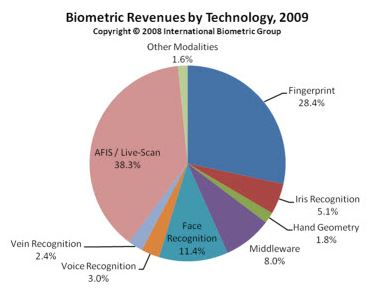
\includegraphics{market.JPG}
	\caption{marché des différentes technologies biométriques}
	\label{fig:market}
\end{figure}

\subsection{Caractéristique biométrique}
 Pratiquement, n'importe quelle caractéristique physiologique ou comportementale peut être considérée comme une caractéristique biométrique, mais elle doit répondre aux critères ci-dessous \citep{Lal} : 
\begin{itemize}
	\item [\textbullet] \textbf{universalité} : la caractéristique doit être présente chez toute personne.
	\item [\textbullet] \textbf{unicité} : pour identifier ou authentifier une personne dans une population, il est nécessaire que la caractéristique biométrique utilisée soit unique à cette personne.
	\item [\textbullet] \textbf{permanence} : la caractéristique doit être suffisamment immuable pendant une période donnée. 
	\item [\textbullet] \textbf{perceptibilité} : la caractéristique doit pouvoir être mesurée quantitativement.  
\end{itemize}
Pour utiliser un système biométrique, plusieurs facteurs doivent être prises en compte au milieu desquels :
 
 \begin{itemize}
	 \item [\textbullet] \textbf{performance} : il s'agit de la fiabilité et de la rapidité de reconnaissance du système, des ressources requises et de l'influence de l'environnement sur le fonctionnement du système.
	\item [\textbullet] \textbf{acceptabilité} : ce facteur traduit la manière dont les gens sont disposés à accepter l'utilisation du système. 
	\item [\textbullet] \textbf{facilité de contournement} : facilité avec laquelle la sécurité du système peut être déjouée.
 \end{itemize}


\subsection{Modes de fonctionnement d'un système biométrique}

Un système biométrique peut fonctionner en trois modes selon le contexte d'utilisation :
\begin{itemize}
	\item [\textbullet] le mode d'\textbf{enrôlement} : c'est une phase d'apprentissage dont le principal but est de recueillir les informations biométriques des individus à identifier. Ces informations sont saisies par un capteur biométrique, puis stockées dans une base de données.
	
	\item [\textbullet] le mode de \textbf{vérification} ou d'\textbf{authentification} : dans ce mode, le système répond à la question \og \textit{Suis-je réellement la personne que je suis en train de proclamer ?}\fg{}\citep{Sou12}. Le système compare les données biométriques saisies avec le modèle biométrique de personne à authentifier (préalablement stockée dans la base de données). C'est une comparaison de type "1 à 1".
	
	\item [\textbullet] le mode d'\textbf{identification} : dans ce mode, le système répond à la question \og \textit{Qui suis-je ?}\fg{}. Une identité est associée à une personne en l'appariant avec l'un des modèles de la base de données. C'est une comparaison de type "1 à N".
\end{itemize}
 Ces différents modes sont résumés dans la figure ci-dessous.
\begin{figure}[htbp]
	\centering
		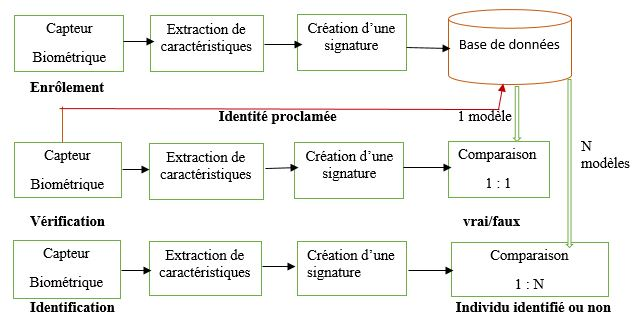
\includegraphics{mode.JPG}
	\caption[modes de fonctionnement d'un système biométrique]{modes de fonctionnement d'un système biométrique (source \cite{Sou12}}
	\label{fig:mode}
\end{figure}

La figure \ref{fig:mode} représente les différents modules qui composent un système biométrique. Leur fonctionnement peut être résumé comme suit :
\begin{itemize}
	\item module capteur biométrique : système d'acquisition équipé d'un terminal de capture biométrique ou capteur biométrique utilisé pour acquérir une caractéristique spécifique de l'utilisateur, par exemple: une caméra ou un microphone dans le cas de la voix.
	\item module d'extraction de données : ayant une image ou une voix en entrée, une étape de segmentation permet d'extraire la caractéristique dont le processus d'authentification/identification a besoin. Par exemple : extraire le visage du fond d'une image dans le cas de l'identification de visage.
	\item module création d'une signature : crée un modèle numérique (ou signature) afin de représenter la 
donnée biométrique acquise. Cette signature est ensuite stockée dans une base de données.
  \item module  comparaison : compare les caractéristiques biométriques d'une personne soumise à contrôle avec les signatures mémorisées.
	\item module base de données : stocke les modèles biométriques des utilisateurs enrôlés.
\end{itemize}



\section{La reconnaissance faciale}
La reconnaissance de visage connaît un grand intérêt auprès de la communauté scientifique. C'est un domaine de recherche aux publications foisonnantes en raison de ses nombreuses applications. Parmi celles-ci les applications de surveillance, de contrôle d'accès dans les lieux publics (aéroports, banques et administrations) et bien d'autres.
Si la reconnaissance de visage apparaît comme un acte naturel et facile chez l'homme, il n'en est pas de même pour un ordinateur. Pour lui, c'est une suite de traitements complexes reposant sur des algorithmes complexes. La reconnaissance automatique de visage s'effectue en trois étapes : la \textbf{détection de visage,} l'\textbf{extraction des caractéristiques du visage} et l'\textbf{identification} et/ou \textbf{vérification}. 


\begin{figure}[htbp]
	\centering
		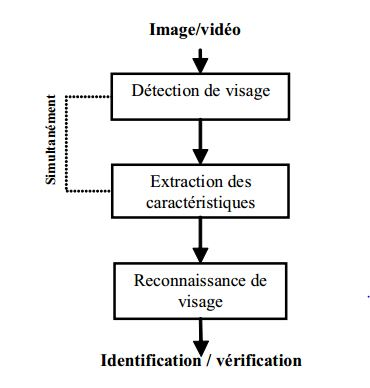
\includegraphics[height=200pt]{etape.JPG}
	\caption{étapes de la reconnaissance faciale}
	\label{fig:etape}
\end{figure}

 
	\subsection{Quelques logiciels gratuits et produits commerciaux}
Le lecteur d'image Picasa de Google intègre une implémentation de la reconnaissance faciale. Il peut associer des visages aux personnes. De même IPHOTO d'Apple utilise un système capable d'étiqueter les visages reconnus sur une photos.  Les systèmes de reconnaissance des visages sont déployés  dans le  transport aérien, le système \og Smart  Gate \fg{} par exemple a été mis en  œuvre  afin d'effectuer  une vérification automatique de l'identité pour l'équipage d'Aéronef traversant la frontière de  l'Australie. Ce dernier  effectue  une  comparaison  entre  le  visage  d'une  personne  à  sa  photographie  de passeport.
Plusieurs entreprises ont orienté leurs activités vers la reconnaissance faciale à l'instar de \og Widget\fg{} par son système \og  Snappy Face\fg{} qui permet d'identifier le visage du propriétaire de l'ordinateur pour sécuriser son accès grâce à une webcam. 

Nous avons ci-dessous quelques produits commerciaux qui font des tâches similaires \citep{Gur}.
\begin{table}[htbp]
	\centering
		\begin{tabular}{|l|l|}
		\hline	Produit commercial & Site Internet \\ 
		\hline	FaceIt from Visionics & http://www.FaceIt.com\\
		\hline	Visage Technology  &http://www.viisage.com\\
		\hline	FaceVACS from Plettac & http://www.plettac-electronics.com\\
		\hline	SpotIt for face composite & http://spotit.itc.it/SpotIt.html\\
		\hline	ImageWare Sofware & http://www.iwsinc.com/ \\
		\hline	Cognitec Systems & http://www.cognitec-systems.de \\
		\hline	Visionsphere Technologies &  http://www.visionspheretech.com/menu.htm\\
		\hline	Biometric Systems & http://www.biometrica.com/ 	\\
		\hline
		\end{tabular}
	\caption{produits commerciaux de reconnaissance faciale}
	\label{tab:produitsCommerciauxDeReconnaissanceFaciale}
\end{table}
\subsection{Pourquoi la reconnaissance de visage?}
 Les caractéristiques  biométriques les plus communément utilisés sont les empreintes digitales. Le premier système d'authentification utilisant les empreintes digitales	fut commercialisé au début des années 80. Une autre caractéristique biométrique beaucoup plus fiable est l'iris car il garde la même texture au cours de la vie. Depuis quelques années, la reconnaissance de visage prend de plus en plus de l'ampleur. Ceci est dû au besoin du monde actuel, mais aussi de ses avantages parmi lesquels on peut citer : 
\begin{itemize}
	\item \textbf{les systèmes de capture} : caméras et appareils photo numériques sont hautement disponibles et à coûts raisonnables, sont faciles à installer et sont acceptables dans les lieux publics.
	\item la\textbf{ passivité} des systèmes à reconnaissance de visages : aucune coopération de la part du sujet à reconnaître n'est nécessaire. Le sujet n'a qu'à se promener devant une caméra pour être identifié. La reconnaissance de visage apparaît donc comme une technique appropriée pour l'identification des individus avec qui on ne peut coopérer, par exemple lors d'une poursuite de suspects.
\end{itemize}
La reconnaissance de visages n'est pas la plus fiable comparée à d'autres systèmes biométriques \cite{Sou12} mais donne de bons résultats lorsque de bonnes approches sont utilisées.


\subsection{Détection de visage}
Le visage humain est la source de diverses informations. Il constitue un vecteur visuel principal à l'identité d'un individu.
La détection de visage est le point d'entrée de tout système de reconnaissance faciale, car pour reconnaître une personne sur une vidéo ou sur une photo, il faut d'abord localiser son visage. Plusieurs travaux de recherches ont été effectués dans le domaine de la détection de visage et diverses méthodes ont été développées (voir section \ref{detection}). L'efficacité d'un système de reconnaissance faciale dépend donc de la technique de détection utilisée.


\subsection{Extraction de caractéristiques du visage}
L'étape d'extraction de caractéristiques constitue le cœur d'un système de reconnaissance, elle consiste à obtenir une représentation plus simple de l'image contenant seulement des informations utiles, discriminantes et non redondantes. Le but est de permettre une meilleure exploitation des données. L'extraction de paramètres peut concerner une région entière du visage (méthode globale) ou un des points particuliers de ses différentes régions caractéristiques comme le nez, la bouche, les coins des yeux\ldots Dans ce second cas, la méthode d'extraction est dite globale. Toutefois, ces deux catégories de méthodes peuvent être utilisées de manière complémentaire (méthodes hybrides).


\subsection{Reconnaissance de visage}
C'est la dernière étape du processus de reconnaissance faciale. Pendant cette phase, les caractéristiques obtenues à l'étape précédente sont utilisées pour créer une signature propre à chaque visage. Cette dernière est ensuite stockée dans une base de données. \`{A} chaque signature de la base correspond donc le visage d'un individu. Ainsi reconnaître un visage consiste donc à extraire sa signature et la mettre en correspondance avec la signature la plus proche dans la base de données. La reconnaissance peut se faire en mode vérification ou identification.

\section{Difficultés de la reconnaissance faciale}
 Si pour le cerveau humain, le processus de reconnaissance de visage est une tâche visuelle de haut niveau, il n'en est pas de même pour un système automatique de reconnaissance faciale. Construire un système capable d'identifier et de reconnaître un visage dans des conditions d'acquisition très variables est un sérieux défi à relever. On distingue deux types de variations associées aux images de visages : inter et intra sujet. La variation inter-sujet n'est rien d'autre que la ressemblance physique entre individu. Quant à la variation intra-sujet, elle est plus vaste et concerne plusieurs facteurs parmi lesquels la variation de l'éclairage, le changement de la position du visage lors de l'acquisition de l'image, etc. Nous analysons ci-dessous les facteurs les plus influents.

\subsection{Changement d'illumination }

La variation d'éclairage (distribution de la source de lumière, son intensité, son spectre) est un facteur très influent dans la tâche de reconnaissance de visage. Elle change l'apparence du visage, rendant ainsi très difficile sa reconnaissance. Adini et al. ont montré de manière expérimentale dans \citep{Adi} avec une base de données de 25 individus que le changement d'un visage dû à l'illumination peut s'avérer plus critique que la différence physique entre individus. 
\begin{figure}[htbp]
	\centering
		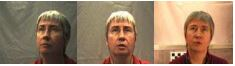
\includegraphics[height=100pt, width=300pt]{illumination.JPG}
	\caption[exemple de variation d'illumination]{exemple de variation d'illumination (source : \cite{Sou12})}
	\label{fig:illumination}
\end{figure}
Ce type de difficulté peut être surmontée par un prétraitement de normalisation et de compensation de l'illumination.
\subsection{Expressions faciales}
L'expression  faciale  est  une  mimique\footnote{jeu de physionomie}  faciale  chargée  de  sens.  Le  sens  peut  être l'expression  d'une  émotion,  un  indice  sémantique  ou une  intonation  dans  la  Langue  des 
Signes. Les  expressions faciales (voir \ref{fig:expression}) entraînent une déformation du visage qui est localisée principalement sur sa partie inférieure. La partie haute reste quasi-invariable et est suffisante pour effectuer une identification. Toutefois, l'expression faciale entraîne une diminution du taux de reconnaissance.
\begin{figure}[htbp]
	\centering
		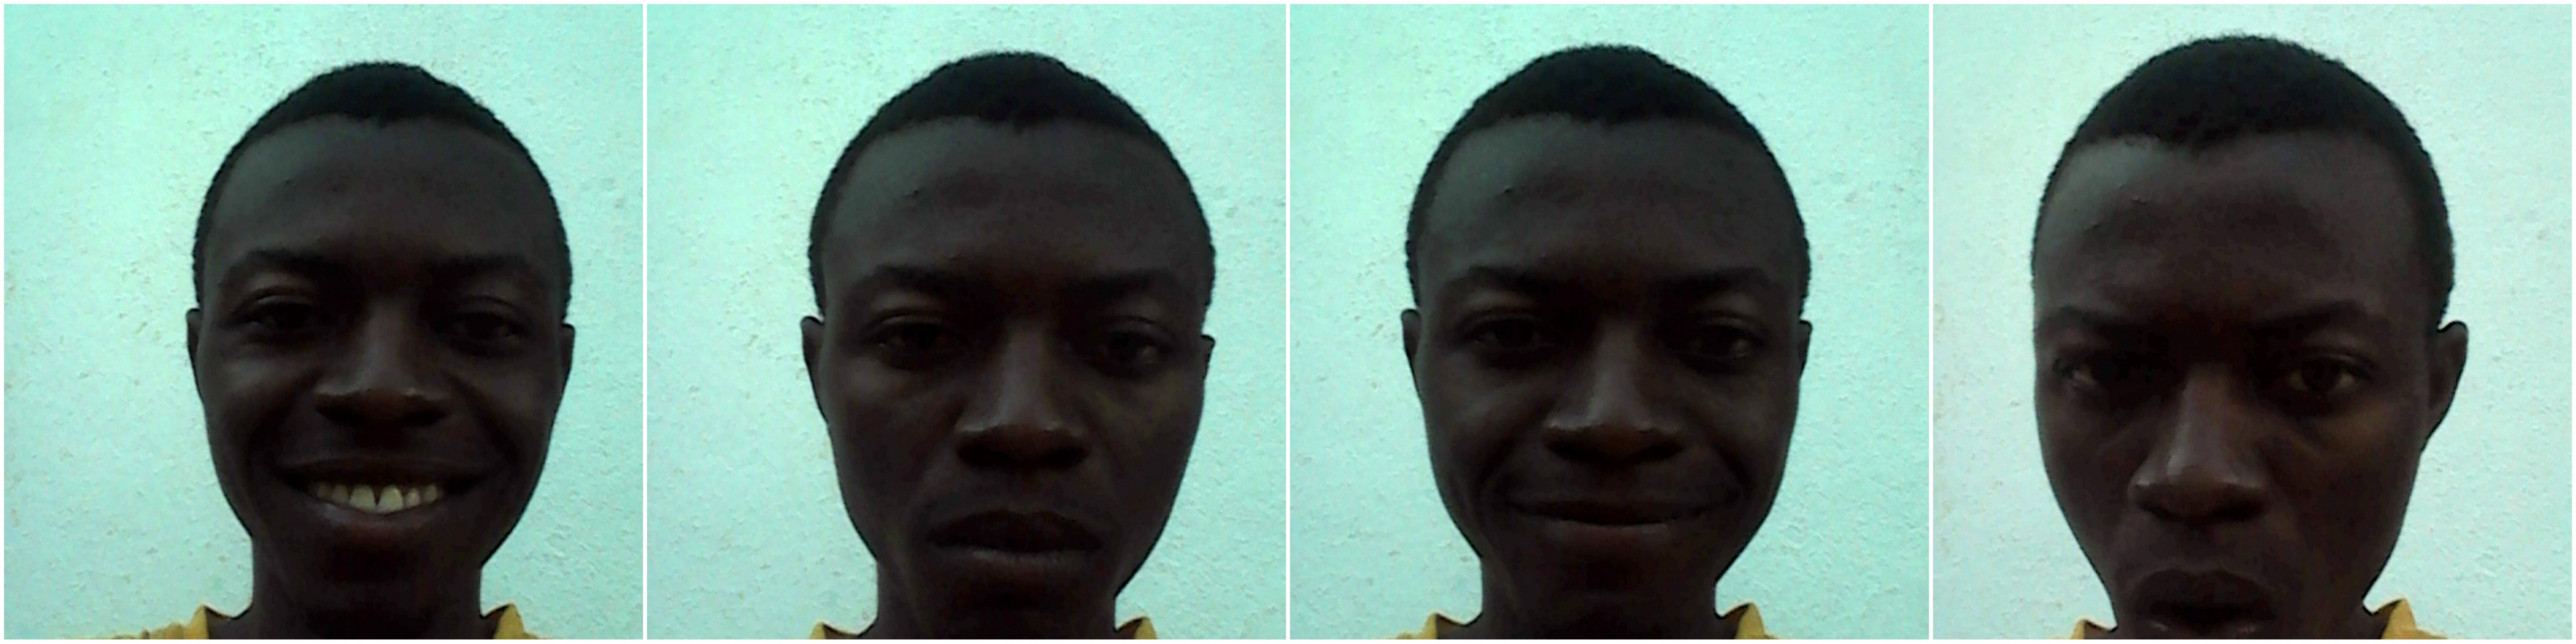
\includegraphics[height=100pt, width=400pt]{expression.jpg}
	\caption{exemple d'expressions faciales}
	\label{fig:expression}
\end{figure}
 
\subsection{Variation de pose}
La variation de pose (figure \ref{fig:pose}) est considérée comme l'un des problèmes majeurs de la reconnaissance de visage. Blackburn et al. dans \citep{Bla01} ont montré cette difficulté en effectuant des tests sur les bases de données FERET\footnote{http://www.itl.nist.gov/iad/humanid/feret/ visité le 24/04/2016} et FRVT\footnote{http://www.frvt.org visité le 24/04/2016}. Selon Blackburn et al., le visage peut être normalisé en détectant au moins  deux  traits  faciaux  (passant  par  les  yeux) quand il est de profil dans le plan image (orientation < 30\degres).  Cependant,  lorsque  la  rotation  est supérieure à 30\degres, la normalisation géométrique n'est plus possible.
\begin{figure}[htbp]
	\centering
		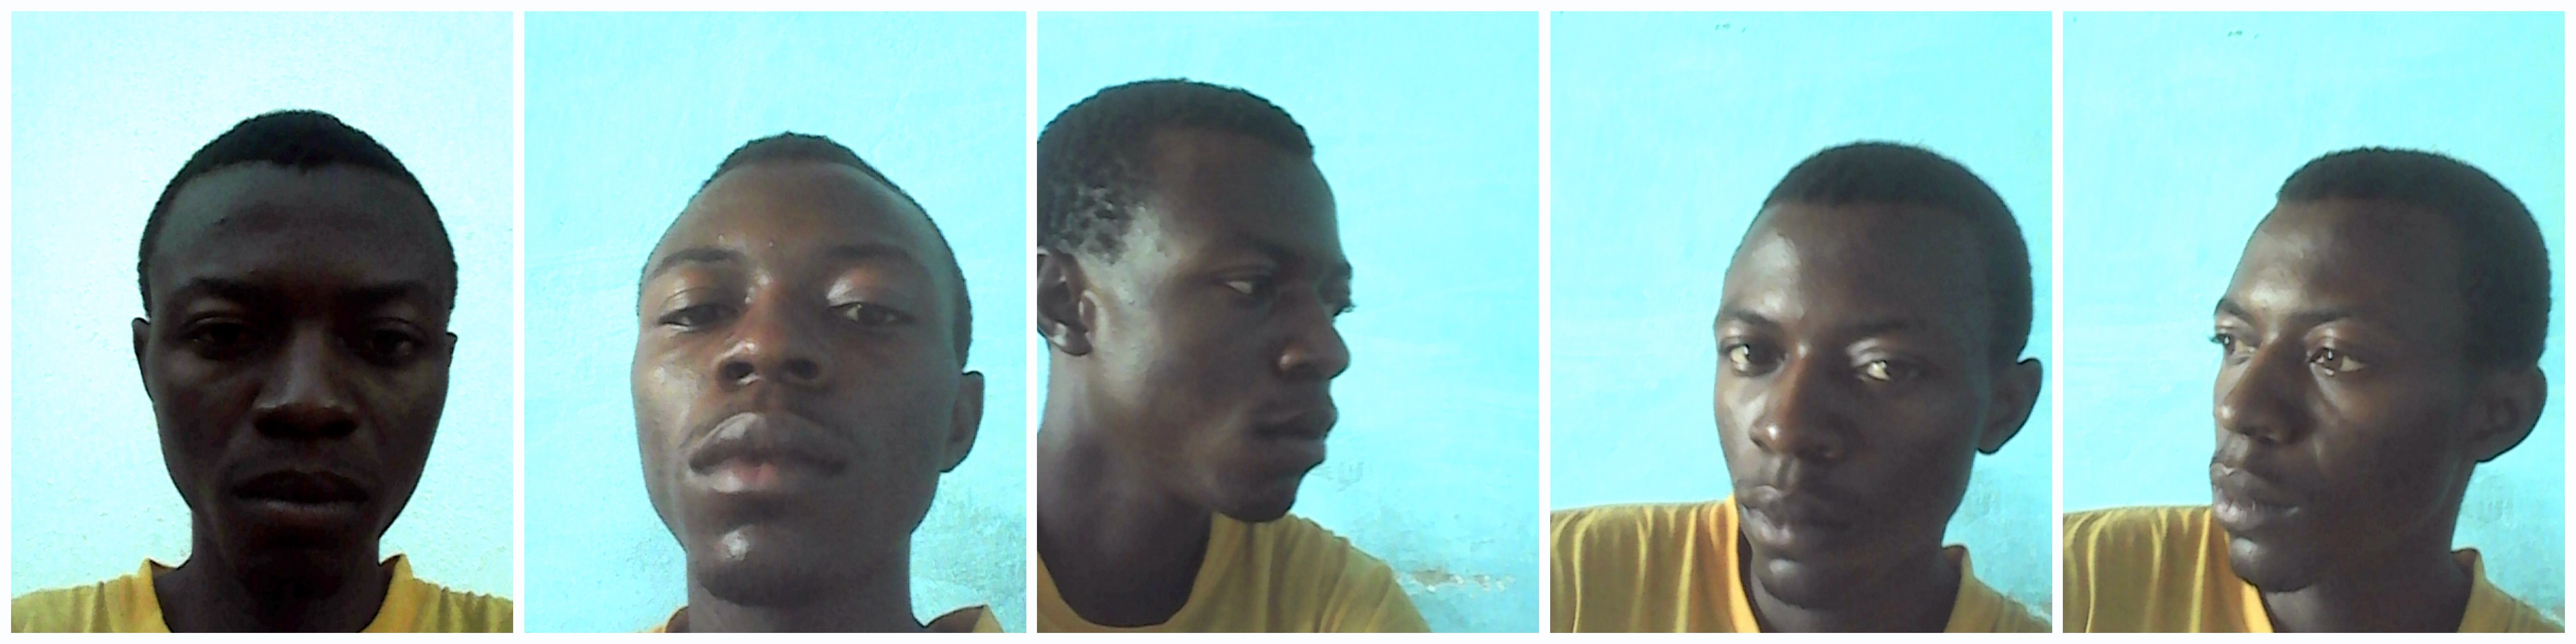
\includegraphics[height=100pt, width=400pt]{pose.jpg}
	\caption{exemple de variation de pose}
	\label{fig:pose}
\end{figure}
 
\subsection{Présence ou absence des composants structurales}
Il s'agit ici des éléments comme la barbe, la moustache, les lunettes, etc. Leur présence sur un visage peut modifier énormément les caractéristiques faciales telles que la forme, la taille ou la couleur du visage entraînant une défaillance ainsi du système de reconnaissance. 

\subsection{Occultations partielles}

Le visage peut être partiellement masqué par des objets dans la scène, ou par le port d'accessoires comme cache-nez, lunettes de soleil, écharpe\ldots Gross et al. dans \cite{Gro} ont étudié l'effet du port de lunettes 
de soleil, et du cache-nez occultant la partie inférieure du visage sur la reconnaissance faciale. Il ressort de cette étude que les performances des algorithmes restent faibles en cas d'occultations partielles de visage.

\subsection{Vrais jumeaux}
Même pour l'homme, reconnaître les vrais jumeaux n'est pas chose facile surtout lorsque l'on est moins familier avec eux. Il est peu probable que la vérification automatique de visage, ne pourra jamais détecter les 
différences très subtiles qui existent entre les vrais jumeaux.


\section{Conclusion}
Nous avons présenté dans ce chapitre les différents systèmes biométriques utilisés pour l'identification/authentification de personnes. L'accent a été mis sur la place qu'occupe la reconnaissance faciale au milieu des techniques biométriques.  Enfin, nous avons mis en évidence les différentes difficultés inhérentes à la reconnaissance automatique de visages. Dans le chapitre suivant, un état de l'art de la reconnaissance faciale sera présenté.
\hspace*{10pt}

\nocite{}